%%%%%%%%%%%%%%%%%%%%%%%%%%%%%%%%%%%%%%%%%%%%%%%%%%%%%%%%%%%%%%%%%%%%%%%%%%%%%%%%%%%%%%%%%%%%%%%%%%%%%%%%%%%%%%%%%%%%%%%%%%%%%%%%%%%%%%%%%%%%%%%%%%%%%%
% 20141006 - Introduction to Operating Systems VO
%%%%%%%%%%%%%%%%%%%%%%%%%%%%%%%%%%%%%%%%%%%%%%%%%%%%%%%%%%%%%%%%%%%%%%%%%%%%%%%%%%%%%%%%%%%%%%%%%%%%%%%%%%%%%%%%%%%%%%%%%%%%%%%%%%%%%%%%%%%%%%%%%%%%%%

\tikzstyle{block} = [rectangle, draw, fill=blue!20, 
    text width=10em, text centered, rounded corners, minimum height=3em]
\tikzstyle{info} = [rectangle, draw, 
    text width=10em, text centered, rounded corners, minimum height=3em]

%fancyhdr
\lhead{IOS VO} 
\rhead{2014-10-06}

%%%%%%%%%%%%%%%%%%%%%%%%%%%%%%%%%%%%%%%%%%%%%%%%%%%%%%%%%%%%%%%%%%%%%%%%%%%%%%%%%%%%%%%%%%%%%%%%%%%%%%%%%%%%%%%%%%%%%%%%%%%%%%%%%%%%%%%%%%%%%%%%%%%%%%

\par{
    \noindent
    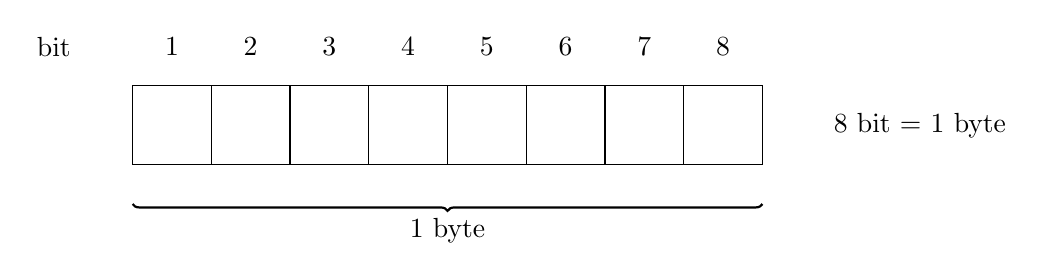
\begin{tikzpicture} 
        \draw (1, 0) rectangle (9, 1);
        \foreach \x in {1, 2, 3, 4, 5, 6, 7} {
            \draw (\x + 1, 0) -- (\x + 1, 1);
            \node at (\x + 1 - 0.5, 1.5) {\x};
        }
        \node at (8.5, 1.5) {8};
        \node at (0, 1.5) {bit};
        \node at (11, 0.5) {8 bit = 1 byte};

        \draw [thick, decoration={ brace, mirror, raise=0.5cm}, decorate]
            (1, 0) -- (9, 0)
            node [pos=0.5,anchor=north,yshift=-0.55cm] {1 byte};
    \end{tikzpicture}
}

\par{
    \noindent
    \underline{Byte-addressing and word-alignment:}
    \par{
        \noindent
        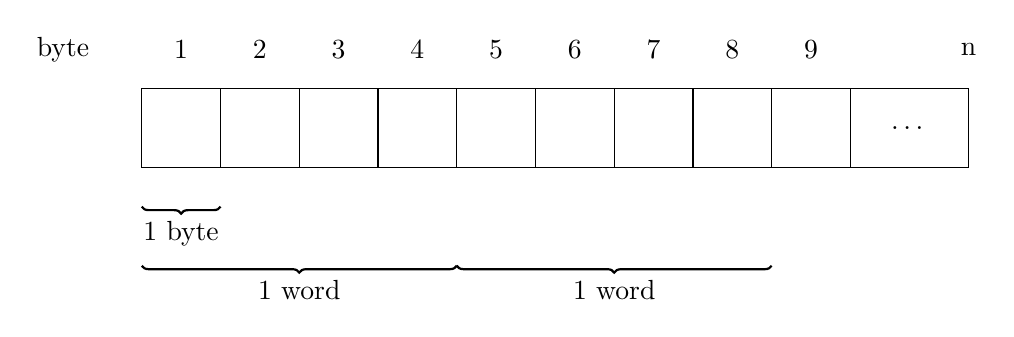
\begin{tikzpicture}
            \draw (1, 0) rectangle (11.5, 1);
            \foreach \x in {1, 2, 3, 4, 5, 6, 7, 8, 9} {
                \draw (\x + 1, 0) -- (\x + 1, 1);
                \node at (\x + 1 - 0.5, 1.5) {\x};
            }
            \node at (10.75, 0.5) {\ldots};
            \node at (11.5, 1.5) {n};
            \node at (0, 1.5) {byte};

            \draw [thick, decoration={ brace, mirror, raise=0.5cm}, decorate]
                (1, 0) -- (2, 0)
                node [pos=0.5,anchor=north,yshift=-0.55cm] {1 byte};
            \draw [thick, decoration={ brace, mirror, raise=0.5cm}, decorate]
                (1, -0.75) -- (5, -0.75)
                node [pos=0.5,anchor=north,yshift=-0.55cm] {1 word};
            \draw [thick, decoration={ brace, mirror, raise=0.5cm}, decorate]
                (5, -0.75) -- (9, -0.75)
                node [pos=0.5,anchor=north,yshift=-0.55cm] {1 word};
        \end{tikzpicture}
    }
}

\par{
    \noindent
    How does the stack access work? \newline
    Why do we do \texttt{R1, R28, -4}? \textbf{Latency}.
}

\par{
    \noindent
    \underline{Implementation of \texttt{void* malloc(int s)}:}
    \par{
        \indent\texttt{LDW 1, 29, 12} \newline
        \indent\texttt{ADD 27, 0, 26} \newline
        \indent\texttt{ADD 26, 26, 1} \newline
    }
    \par{
        \noindent
        \texttt{s}: \texttt{R1 = sum[R29 + 12]} \newline
        Because you do not have access to registers in \texttt{C$^*$}, the above behavior has to be implemented in assembler. \newline
        \texttt{malloc} is pat of the (g)libc and is a de facto feature of operating systems nowadays.
    }
    \par{
    	\noindent\underline{Implementation of \texttt{int getchar()}:} \newline
        \indent\texttt{RDC 0, 0, 27}
    }
    \par{
    	\noindent\underline{Implementation of \texttt{void putchar(int c)}:} \newline
        \indent\texttt{LDW 1, 29, 12} \newline
        \indent\texttt{WRC 0, 0, 1}
    }
    \par{
    	\noindent
    	Reads the next character from the stream. \newline
    	\texttt{R27 = getchar();} \newline
    	Streams: \texttt{stdin}, \texttt{stdout}, \texttt{stderr}
    }
    \par{
        \noindent
        \begin{figure}[H]
            \centering
            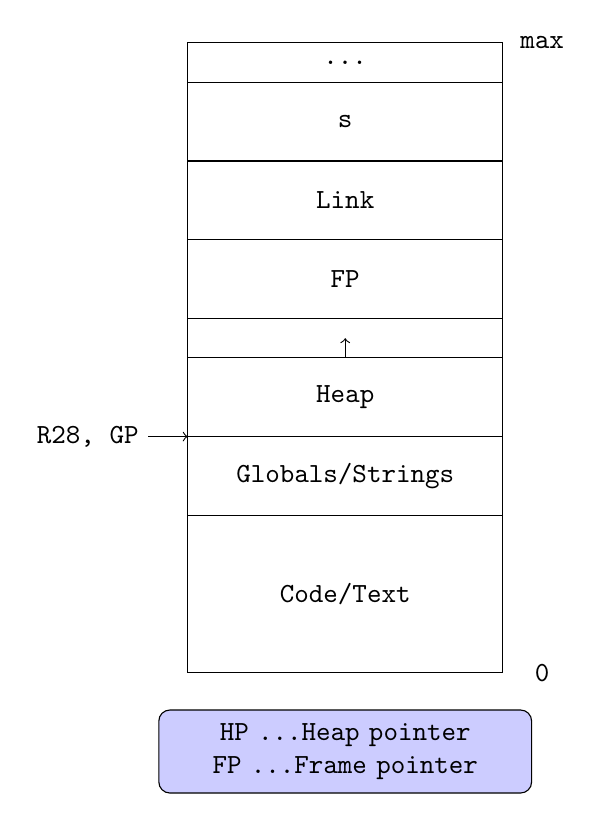
\begin{tikzpicture}
                \draw (2, 1.5) rectangle (6, 9.5);
                
                \node at (6.5, 1.5) {\texttt{0}};
                \node at (6.5, 9.5) {\texttt{max}};

                \draw (2, 9) -- (6, 9);
                \node at (4, 9.25) {\texttt{\ldots}};
                
                \draw (2, 8) -- (6, 8);
                \node at (4, 8.5) {\texttt{s}};

                \draw (2, 7) -- (6, 7);
                \node at (4, 7.5) {\texttt{Link}};

                \draw (2, 6) -- (6, 6);
                \node at (4, 6.5) {\texttt{FP}};

                \draw (2, 3.5) -- (6, 3.5);
                \node at (4, 2.5) {\texttt{Code/Text}};
                
                \draw (2, 4.5) -- (6, 4.5);
                \node at (4, 4) {\texttt{Globals/Strings}};

                \draw (2, 5.5) -- (6, 5.5);
                \node at (4, 5) {\texttt{Heap}};
                \draw[->] (4, 5.5) -- (4, 5.75);
                \draw[<-] (2, 4.5) -- (1.5, 4.5) node[left]{\texttt{R28, GP}};

                \node[block] at (4, 0.5) [text width = 4.5cm]{\texttt{HP \ldots Heap pointer FP \ldots Frame pointer}};
            \end{tikzpicture}
            \caption{Memory layout revisited}
            \label{fig:memorylayout}
    	\end{figure}
    }
    \par{
	    \noindent
	    \textbf{F2}
	}
	\par{
	    \noindent
	    \begin{tabular}{llll}
	        \hline
	        Instruction 	& Semantics 						& Additional information	\\
	        \hline
	        \hline
	        \texttt{RDC c}  &   \texttt{reg[c] = getchar();}	& 							\\
	                        &   \texttt{pc:=pc+4;}				&              				\\
	        \texttt{WRC c}  &   \texttt{putchar(reg[c]);}		& 							\\
	                        &   \texttt{pc:=pc+4;}				& 							\\
	        \hline
	    \end{tabular}   
	}
	\par{
		\noindent
		Why is it so hard to implement \texttt{RDC} and \texttt{WRC} on application level? Because operating systems stuff is self-referential!
		\begin{figure}[H]
			\centering
			\begin{tikzpicture}
				\node[draw, minimum width = 4cm, minimum height = 2cm] (processor) at (0, 0) {processor};
				\node[draw, minimum width = 4cm, minimum height = 2cm, above = -0.015 of processor] (appC) {application in \texttt{C$^*$}};

				\node[right = 0 of processor.north east, text width = 0.5em] (os_t) {OS, DLX};
			\end{tikzpicture}
			\caption{Application and processor}
            \label{fig:appandproc}
		\end{figure}
	}
	\par{
		\noindent
		How does I/O work on a processor?
		\begin{figure}[H]
			\centering
			\begin{tikzpicture}
				\node[draw, minimum width = 3cm, minimum height = 3cm] (processor) at (0, 0) {};
				\node[draw, right = 0.125 of processor.west] (cpu) {CPU};
				\node[draw, above left = 0.25 and 0.125 of processor.east] (in1) {};
				\node[draw, below left = 0.25 and 0.125 of processor.east] (in2) {};
				\node[above = 0.125 of processor.north east] (data_t) {data};
				\node[below = 0.125 of processor.south east] (control_t) {control};
				\draw[dashed] (data_t.south) -- (in1.north);
				\draw[dashed] (control_t.north) -- (in2.south);

				\node[draw, right = 1 of processor, minimum width = 1.75cm, minimum height = 1.2cm] (rs232) {};
				\node[draw, below right = 0.125 and 0.125 of rs232.north west] (rs232_1) {\tiny{1}};
				\node[draw, right = 0.125 of rs232_1] (rs232_2) {\tiny{2}};
				\node[draw, right = 0.125 of rs232_2] (rs232_3) {\tiny{3}};
				\node[draw, below = 0.125 of rs232_1] (rs232_4) {\tiny{4}};
				\node[draw, right = 0.125 of rs232_4] (rs232_5) {\tiny{5}};
				\node[draw, right = 0.125 of rs232_5] (rs232_6) {\tiny{6}};
				\node[below = 0 of rs232.south] (rs232_t) {RS232};
				\node[right = 0 of rs232.east] (ascii_t) {ASCII};

				\draw[<->, >=stealth, thick] (processor.east) -- (rs232.west);
			\end{tikzpicture}
			\caption{I/O on a processor}
            \label{fig:ioproc}
		\end{figure}
	}
}

\par{
	\noindent\underline{Computability \& Complexity of algorithms}
	\par{
		\noindent
		What is the minimal machine that is still universal?
		\begin{itemize}
			\item{
				RISC: Reduced Instruction Set Computer \newline
				Has separate instructions to load/store \& compute. \newline
				E.g. ARM, MIPS, SPARC, \ldots
			}
			\item{
				CISC: Complex Instruction Set Computer \newline
				More complex instructions which load, compute \& store in a single instruction. \newline
				E.g. x86
			}
		\end{itemize}
		RISC vs. CISC $\leftrightarrow$ Compiler vs. processor.
	}
	\par{
		\noindent
		OISC/URISC: One/Ultimate Reduced Instruction Set Computer \newline\newline
		\texttt{SUBLEQ a, b, c}: Subtraction less or equal \newline
		\indent\texttt{mem[b] := mem[b] - mem[a];} \newline
		\indent\texttt{if mem[b] $\le$ 0 goto c;} \newline
		\indent\texttt{else pc := pc + 4;}
	}
	\par{
		\noindent
		\begin{figure}[H]
			\centering
			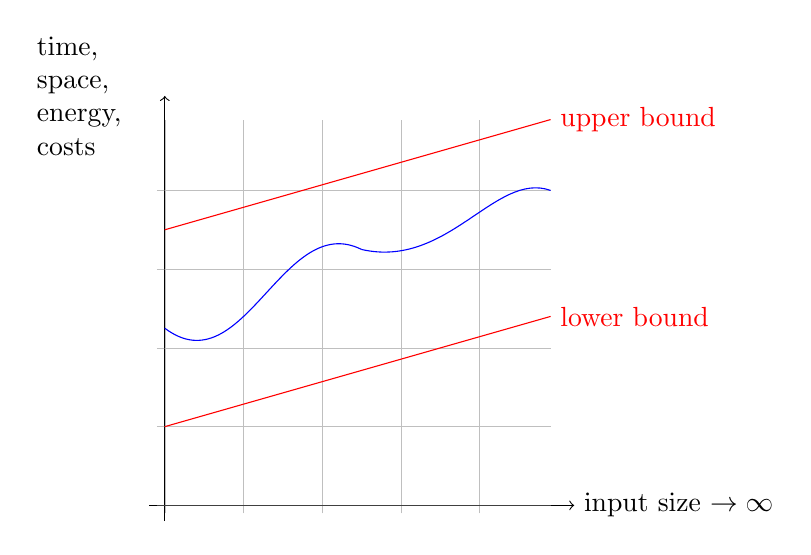
\begin{tikzpicture}
				\draw[->] (-0.2, 0) -- (5.2, 0) node[right] {input size $\rightarrow \infty$};
				\draw[->] (0, -0.2) -- (0, 5.2) node[left, text width = 1.5cm] {time, space, energy, costs};
				\draw[very thin, color = gray, opacity = 0.5] (-0.1, -0.1) grid (4.9, 4.9);

				\draw[color = red] (0, 3.5) -- (4.9, 4.9) node[right] {upper bound};
				\draw[color = red] (0, 1) -- (4.9, 2.4) node[right] {lower bound};
				\draw[color = blue] (0, 2.25) .. controls (1, 1.5) and (1.5, 3.75) .. (2.5, 3.25);
				\draw[color = blue] (2.5, 3.25) .. controls (3.6, 3) and (4.2, 4.25) .. (4.9, 4);
			\end{tikzpicture}
			\caption{Asymptotic computational complexity [1]}
			\label{fig:asymcompl1}
		\end{figure}
		\begin{figure}[H]
			\centering
			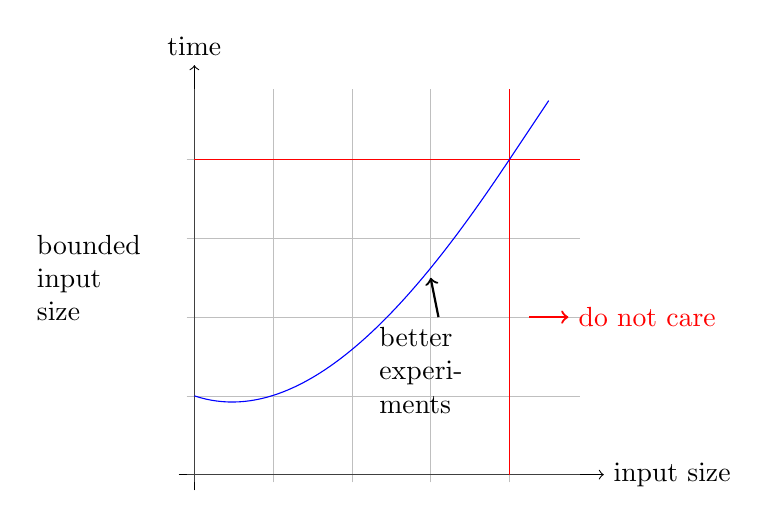
\begin{tikzpicture}
				\draw[->] (-0.2, 0) -- (5.2, 0) node[right] {input size};
				\draw[->] (0, -0.2) -- (0, 5.2) node[above] {time};
				\draw[very thin, color = gray, opacity = 0.5] (-0.1, -0.1) grid (4.9, 4.9);

				\draw[color = red] (0, 4) -- (4.9, 4) node[right] {};
				\draw[color = red] (4, 0) -- (4, 4.9) node[right] {};
				\draw[color = blue] (0, 1) .. controls (1.5, 0.5) and (3, 2.5) .. (4, 4);
				\draw[color = blue] (4, 4) -- (4.5, 4.75);
				\node[text width = 1cm] at (-1.5, 2.5) {bounded input size};
				\draw[->, thick] (3.1, 2) node[below, text width = 1.5cm] {better experiments} -- (3, 2.5);
				\draw[->, thick, color = red] (4.25, 2) -- (4.75, 2) node[right] {do not care};
			\end{tikzpicture}
			\caption{Asymptotic computational complexity [2] (for operating systems)}
			\label{fig:asymcompl2}
		\end{figure}
		\begin{figure}[H]
			\centering
			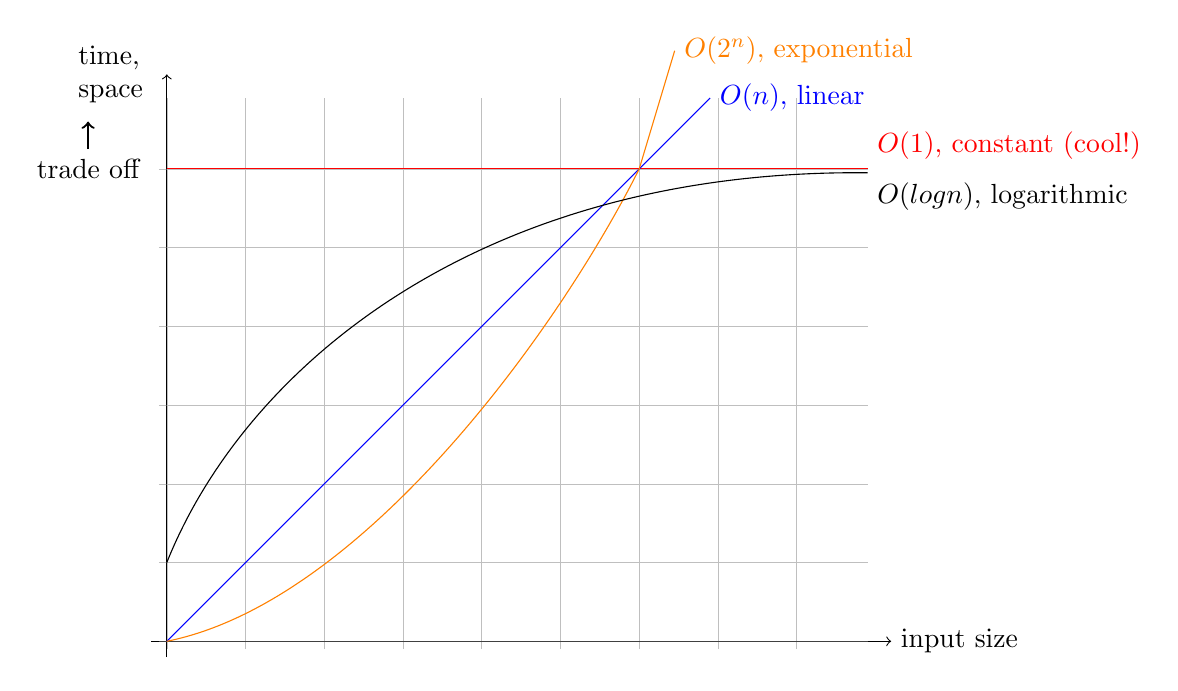
\begin{tikzpicture}
				\draw[->] (-0.2, 0) -- (9.2, 0) node[right] {input size};
				\draw[->] (0, -0.2) -- (0, 7.2) node[left, text width = 1cm] {time, space};
				\draw[very thin, color = gray, opacity = 0.5] (-0.1, -0.1) grid (8.9, 6.9);

				\draw[color = red] (0, 6) -- (8.9, 6) node[above right] {$O(1)$, constant (cool!)};
				\draw[color = blue] (0, 0) -- (6.9, 6.9) node[right] {$O(n)$, linear};
				\draw[color = orange] (0, 0) .. controls (2.5, 0.5) and (5, 4) .. (6, 6);
				\draw[color = orange] (6, 6) -- (6.45, 7.5) node[right] {$O(2^n)$, exponential};
				\draw[color = black] (0, 1) .. controls (1, 3.5) and (4, 6) .. (8.9, 5.95) node[below right = 0] {$O(log n)$, logarithmic};
				
				\draw[->, thick] (-1, 6.25) node[below] {trade off} -- (-1, 6.6);
			\end{tikzpicture}
			\caption{Big O notation (upper bound)}
			\label{fig:bigonotation}
		\end{figure}
	}
	\par{
		\noindent\underline{Big O notation (upper bound): $O(\#bits)$}
		\par{\noindent$O(\#bits) = O(\#bytes) = O(\#char) = O(\#instructions) = O(\#objects)$}
	}
	\par{
		\noindent\underline{Numeric representation}
		\par{
			\noindent
			unary: $\underbrace{||||| ||||| ||||| |0}_{16}$, binary: $\underbrace{1 0000}_{16}$, octal: $\underbrace{20}_{16}$, decimal: $\underbrace{16}_{16}$, hexadecimal: $\underbrace{10}_{16}$ \newline
			Exponential reduction from unary to binary representation: $1 + n = \lfloor log_2 n\rfloor + 1$ \newline
			The main difference ist the denseness of the representations.
		}
	}
	\par{
		\noindent
		\texttt{fib(n) \{} \newline
		\indent\texttt{if $n \le 2$} \newline
		\indent\indent\texttt{return n;} \newline
		\indent\texttt{else} \newline
		\indent\indent\texttt{return (fib($n - 1$) + fib($n - 2$));} \newline
		\texttt{\}}
	}
	\par{
		\noindent
		This implementation has a worst-case time complexity of $O(2^n)$. Thus, \texttt{fib(7)} will terminate correctly but something like \texttt{fib(1024)} will not terminate correctly on most systems. \newline
		There exists another implementation of the Fibonacci numbers using dynamic programming. This implementation has a logarithmic worst-case time complexity.
	}
	\par{\noindent $log(n) \cdot log_d(2) = log_d(n)$}
	\clearpage
	\par{
		\noindent\underline{From Turing to digital:}
		\begin{figure}[H]
			\centering
			\begin{tikzpicture}
				\node[text width = 3.4cm] at (6, 0) (program_data) {Program = data, Data = addresses};
				\node[above left = 1 and 2 of program_data] (von_neumann) {Von Neumann architecture};
				\node[above = 2 of program_data] (stored_program_computer) {Stored program computer};
				\node[above = 1 of von_neumann] (universal_turing_machine) {Universal Turing Machine};
				\node[above right = 2 and 1 of universal_turing_machine] (algorithm) {Algorithm};
				\node[above = 2 of universal_turing_machine] (turing_machine) {Turing Machine};

				\draw[<->, >=stealth, thick] (program_data.west) -- (von_neumann.south);
				\draw[<-, >=stealth, thick] (program_data.north) -- node[right] {\textit{memory}} (stored_program_computer.south);
				\draw[<-, >=stealth, thick] (von_neumann.north) -- node[left] {\textit{hardware}} (universal_turing_machine.south);
				\draw[<->, >=stealth, thick] (stored_program_computer.west) -- (universal_turing_machine.east);
				\draw[<-, >=stealth, thick] (stored_program_computer.north) -- node[right] {\textit{software}} (algorithm.south);
				\draw[<-, >=stealth, thick] (universal_turing_machine.north) -- node[left] {\textit{first interpreter}} (turing_machine.south);
				\draw[<->, >=stealth, thick] (algorithm.west) -- (turing_machine.east);
 			\end{tikzpicture}
			\caption{From Turing to digital}
			\label{fig:fromturingtodigital}
		\end{figure}
	}
	\par{
		\noindent\underline{TM:}
		\begin{figure}[H]
			\centering
			\begin{tikzpicture}[zero/.style = {draw}]
				\node at (2, 2) (empty_1) {\vphantom{1}};
				\foreach \i [count = \ii from 1] in {2, ..., 5}{
					\node[right = -0.015 of empty_\ii] (empty_\i) {\vphantom{1}};
				}
				
				\node[zero, right = -0.015 of empty_5] (zero_1) {0};
				\foreach \i [count = \ii from 1] in {2, ..., 12}{
					\node[zero, right = -0.015 of zero_\ii] (zero_\i) {0};
				}

				\node[right = -0.015 of zero_12] (empty_6) {\vphantom{1}};
				\foreach \i [count = \ii from 6] in {7, ..., 10}{
					\node[right = -0.015 of empty_\ii] (empty_\i) {\vphantom{1}};
				}

				\draw (empty_1.north west) -- (empty_10.north east);
				\draw (empty_1.south west) -- (empty_10.south east);

				\node[above = 0 of empty_1] (tape_t) {tape};
				\draw[<-, >=stealth] (empty_10.east) -- ++(1, 0.5) node[right] {$\infty$};
				\draw[<-, >=stealth] (zero_6.south) -- node[right = 0.25] {\textit{write}} node[left = 0.25] {\textit{read}} ++(0, -0.5) node[below] {left $\leftarrow$ head $\rightarrow$ right};
			\end{tikzpicture}
			\caption{TM read/write}
			\label{fig:tmrw}
		\end{figure}
	}
	\par{
		\noindent\underline{Program:}
		\begin{figure}[H]
			\centering
			\begin{tikzpicture}[>=stealth', shorten >= 1pt, auto, node distance = 3cm, scale = 1, transform shape]
				\node[initial, state] (a) {A};
				\node[state, right of = a] (b) {B};
				\node[state, below right of = a] (c) {C};
				\node[state, accepting, right of = c] (h) {H};

				\path[->]	(a) edge[left, bend right] node[below] {0/1, R} (b)
							(b) edge[right, bend right] node[above] {0/1, L} (a)
							(b) edge[loop right] (b)
							(a) edge[below, bend right] (c)
							(c) edge[above, bend right] (b)
							(c) edge[right] (h)
				; 
			\end{tikzpicture}
			\caption{Busy beaver (3 states)}
			\label{fig:busybeaver}
		\end{figure}
	}
}